\chapter{Introducci\'on}

\section{Render}
El render es una de las areas de la computacion grafica que se encarga de
traducir estructuras de datos o funciones a pixeles en la pantalla para crear imagenes
en bidimensionales o tridimensionales.
With the increasing sophistication of computer graphics since the 1970s, it has become
a more distinct subject.

Es un area nacida en ..... que siguio desarrollandose con ...... hasta ser parte clave
de industrias como las peliculas de animacion, efectos especiales, arquitectura, disenho
y videojuegos Un motor de render. 

Se pueden clasificar en fotorealistas o no fotorealistas, segun su intencion o no deimitar la realidad. 
NPR está inspirado en estilos artísticos como la pintura , el dibujo, ilustración técnica, y los dibujos animados.
NPR ha aparecido en películas y videojuegos en forma de sombreado toon, así como en la visualización científica,
ilustración arquitectónica y animación experimental. Los motores no realistas trabajan con diferentes tecnicas,
como gooch shading o el cel shading.

Por otra parte, los motores fotorealistas son los mas frecuentes en la industria por sus multiples aplicaciones, de simular el comportamiento de la luz en una escena 2D o 3D. 
Es un programa que se encarga de generar imagenes en 2D o 3D. Para ello carga una escena virtual
A scene file contains objects in a strictly defined language or data structure; it would contain geometry, viewpoint, texture, lighting, and shading information as a description of the virtual scene.
The data contained in the scene file is then passed to a rendering program to be processed and output to a digital image or raster graphics image file. 
If a scene is to look relatively realistic and predictable under virtual lighting, the rendering software should solve the rendering equation

\singlespacing

\begin{figure}[H]
\setlength{\fboxsep}{0pt}
\fbox{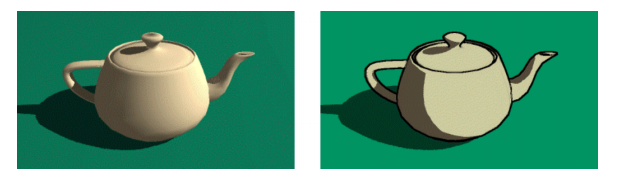
\includegraphics[width=0.99\linewidth]{images/cel-shading.png}}
\caption{
    A teapot model rendered photorealistically (left) and using cartoonlooking method (right), which later
    became known as cel-shading.\autocite{decaudinnpr}
}
\singlespacing
\end{figure}

\section{Unidades b\'asicas radiom\'etricas}
    Flujo radiante es la medida de la potencia de una radiación electromagnética. Es la energía que
    transportan las ondas por unidad de tiempo.
    \begin{equation}
        \Phi_e = \dfrac{d{Q_e}}{dt}
    \end{equation}
    \singlespacing

    La irradiancia (E) es la densidad del flujo radiante con respecto a un \'area.
    La irradiancia para un punto dentro de una superficie con \'area A es expresada como:
    \begin{equation}
        E = \dfrac{d\Phi}{dA}
    \end{equation}
    Cuando este flujo de radiancia se mide en direcci\'on contraria, de salida, se llama emitancia (M)
    \singlespacing

    La intensidad (I) describe la distribuci\'on direccional de la luz. En su definici\'on se incluye
    el concepto de \'angulo s\'olido. Un \'angulo s\'olido puede ser visualizado como la extensi\'on
    de un \'angulo sobre una esfera y su unidad es el estereorradi\'an. Una esfera tiene un \'angulo
    s\'olido de 4$\pi$. La intensidad se define como la densidad de flujo radiante por \'angulo s\'olido
    $\omega$
    \begin{equation}
        I = \dfrac{d\Phi}{d\omega}
    \end{equation}
    \singlespacing

    La radiancia (L) combina las ideas de irradiancia e intensidad y se define como la densidad de flujo
    radiante con respecto al \'area y \'angulo s\'olido.
    $\omega$
    \begin{equation}
        L = \dfrac{d^2\Phi}{dA_{proj}d\omega}
    \end{equation}
    $A_proj$ representa la proyecci\'on de $dA$ sobre un plano perpendicular al \'angulo s\'olido
    $\omega (dA_{proj} = dA|cos\theta|)$. Podemos pensar en la radiancia como la medida de energía a
    trav\'es de un \'unico rayo.
    \singlespacing

\section{Ecuaci\'on de render}
    

\section{Motores online y offline}
    \subsection{Motores offline}
    El motor de render offline de Seddi es un ray tracer, un algoritmo que simula el camino de los rayos de luz que llegan a la camara directamente desde las fuentes de luz o rebotados desde las superficies de los elementos que componen un escena 3D. El objetivo es estimar una intensidad y frecuencia de onda a cada pixel visible desde el punto de vista de la camara.
    Para ello, por cada pixel de la matriz 2D de la pantalla, se lanza un rayo para comprobar que elemento de la escena debe ser mostrado ahi. Desde ese punto de una superficie se vuelven a lanzar nuevos rayos para simular como reacciona a su encuentro con otros elementos.
    Esta tecnica fue introducida por primera vez por Arthur Appel, en 1969, en Some Techniques for Shading Machine Renderings of Solidsy presentaba  "results in the automatic shading of line drawings". Ya en 1979, Turner Whitted presento el paper  An Improved Illumination Model for Shaded Display en el que se introducian tecnicas para capturar fenomenos fisicos de la luz como la reflexion, , refraccion o sombras.
    With Whitted’s technique, when a ray encounters an object in the scene, the color and lighting information at the point of impact on the object’s surface contributes to the pixel color and illumination level. If the ray bounces off or travels through the surfaces of different objects before reaching the light source, the color and lighting information from all those objects can contribute to the final pixel color.
    Another pair of papers in the 1980s laid the rest of the intellectual foundation for the computer graphics revolution that upended the way movies are made. (Cook? PT?)
    In 1984, Lucasfilm’s Robert Cook, Thomas Porter and Loren Carpenter detailed how ray tracing could incorporate a number of common filmmaking techniques — including motion blur, depth of field, penumbras, translucency and fuzzy reflections — that could, until then, only be created with cameras.
    
    un sistema recursivo basado en la tecnica de ray-tracing.
    El ray-tracing es un algoritmo introducido por  Arthur Appel, in 1969, in ” que trata de samplear los valores de radiancia de las superficies que conforman una escena 3D.
    Ray tracing is eye-oriented process that needs walking through each pixel looking for what object should be shown there, which is also can be described as a technique that follows a beam of light (in pixels) from a set point and simulates how it reacts when it encounters objects.
    Consider the picture : figure 4. Ray traced graphics would start at your “eye”, actually it’s camera here. And then the shooting ray from each pixel of the image plane will follow your line of sight to the scene object, and then follow the path of light from the intersected object back to the light source.
    
    The next major breakthrough came a decade later. In a 1979 paper, An Improved Illumination Model for Shaded Display, Turner Whitted, now with NVIDIA Research, showed how to capture reflection, shadows and refraction.
    With Whitted’s technique, when a ray encounters an object in the scene, the color and lighting information at the point of impact on the object’s surface contributes to the pixel color and illumination level. If the ray bounces off or travels through the surfaces of different objects before reaching the light source, the color and lighting information from all those objects can contribute to the final pixel color.
    Another pair of papers in the 1980s laid the rest of the intellectual foundation for the computer graphics revolution that upended the way movies are made. (Cook? PT?)
    In 1984, Lucasfilm’s Robert Cook, Thomas Porter and Loren Carpenter detailed how ray tracing could incorporate a number of common filmmaking techniques — including motion blur, depth of field, penumbras, translucency and fuzzy reflections — that could, until then, only be created with cameras.
    
    Por su parte, el la tecnica de path tracing es una forma particular de ray-tracing en la que se utiliza multiple importance sampling, ...
    in path tracing , instead of sending out one ray it sends out tens, hundreds or even thousands of rays for each pixel to be rendered. When it hits a surface it doesn’t trace a path to every light source, instead it bounces the ray off the surface and keeps bouncing it until it hits a light source or exhausts some bounce limit. It then calculates the amount of light transferred all the way to the pixel, including any color information gathered from surfaces along the way. It then averages out the values calculated from all the paths that were traced into the scene to get the final pixel color value.  Besides, now most of softwares use path tracing as the prior rendering technique*
    Firstly, path tracing is an evolution of classic Turner Whitted raytracing. As we mentioned before that for classic ray tracing the rays will increase exponential. Path tracing provides a solution to that. For each pixel, instead of shooting only one ray, it shoots off multiple rays in a random direction. 
    path tracing can be used to solve more complex lighting situations (with diffuse inter-reflection or caustics) through the use of Monte Carlo integration to solve an integral equation which represents light transport within a scene 
    \singlespacing

    \subsection{Motores online}
        Es el motor de tiempo real que permite la interaccion del usuario.
        Los motores de render online utilizan la tecnica de rasterizacion. 
        rasterization is simply the process of computing the mapping from scene geometry to pixels* 
        The GPU will tell the game to create a 3D image out of small shapes, most often triangles. These triangles are turned into individual pixels and then put through a shader* 
        With rasterization, objects on the screen are created from a mesh of virtual triangles, or polygons, that create 3D models of objects. In this virtual mesh, the corners of each triangle — known as vertices — intersect with the vertices of other triangles of different sizes and shapes. A lot of information is associated with each vertex, including its position in space, as well as information about color, texture and its “normal,” which is used to determine the way the surface of an object is facing.*
        Computers then convert the triangles of the 3D models into pixels, or dots, on a 2D screen. Each pixel can be assigned an initial color value from the data stored in the triangle vertices.*

        Further pixel processing or “shading,” including changing pixel color based on how lights in the scene hit the pixel, and applying one or more textures to the pixel, combine to generate the final color applied to a pixel.*

        En Computer Graphics, la tecnica del shading permite mejorar la percepcion de
        los volumenes en 3D. Con el aumento de la capacidad de computacion estas tenicas
        han evolucionado mucho en un breve periodo de tiempo.\sidenote{Is this correct?}\sidenote{I'm unsure about also!}
        Las primeras aportaciones el campo fueron durante los anhos 70 por parte de Bui
        Tuong Phong, Henri Gouroud y Jim Blinn con sus modelos de shading: Phong\autocite{phong}, Gouraud\autocite{gouraud}
        y Blinn-Phong\autocite{blinnphong}. Estos algoritmos permiten, a partir de la posicion de la luz, y la
        position de la camara, dar una estimacion de la cantidad de luz emitida por una
        superficie.
    \singlespacing

\begin{figure}[H]
\setlength{\fboxsep}{0pt}
\fbox{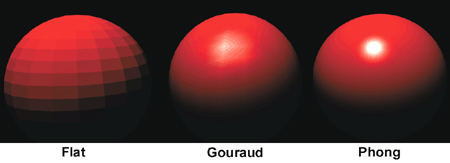
\includegraphics[width=0.99\linewidth]{images/gouroud-phong-flat.jpg}}
\caption{A boat.}
\singlespacing
\end{figure}

\todo[inline]{
    TODO: hablar sobre matriz de perspectiva de
    \href{http://www.cs.uns.edu.ar/cg/clasespdf/p465carlbom.pdf}
    {Ingrid Carlbon}
}

\todo[inline]{
    Siguientes a\~nos: antialising, sombras, multinucleo aparicion GPUs,
    raytracing...
    \href{https://ohiostate.pressbooks.pub/graphicshistory/back-matter/cg-historical-timeline/\#1970}
    {fuente}
}

\todo[inline]{
    Blinn’s law: “as technology advances, rendering time remains constant.” 
    from
    \href{http://www.pbr-book.org/3ed-2018/Introduction/A_Brief_History_of_Physically_Based_Rendering.html}
    {here}
}

\todo[inline]{
    Blinn's law: James Blinn first pointed out, in animation, rendering time remains
    constant, even as computers get faster. An artist gets accustomed to waiting a
    certain number of hours for an image to render, so as hardware improves, instead
    of using it to save time, he employs it to render more complex graphics. from
    \href{https://nevalalee.wordpress.com/2011/08/09/blinns-law-and-the-paradox-of-efficiency/}
    {here}
}

\todo[inline]{
    TODO: Esquema evolucion en el tiempo del shading: phong, blinn-phong
}

\todo[inline]{
    PBR, PBM, PBS

    Physically Based Rendering PBR is a method of shading and rendering that provides a more
    accurate representation of how light interacts with surfaces. It is referred to as Physically
    Based Rendering PBR or Physically Based Shading PBS. Depending on what aspect of the pipeline
    is being discussed, PBS is usually specific to shading concepts and PBR is specific to rendering
    and lighting. However, both terms describe the process of representing assets from a physically
    accurate standpoint.

    Physically based rendering PBR is an approach in computer graphics that seeks to render graphics
    in a way that more accurately models the flow of light in the real world. Many PBR pipelines have
    the accurate simulation of photorealism as their goal. Feasible and quick approximations of the
    bidirectional reflectance distribution function and rendering equation are of mathematical
    importance in this field. Photogrammetry may be used to help discover and encode accurate optical
    properties of materials. Shaders may be used to implement PBR principles.\\
    What are the benefits?

    As artists, we can view the benefits of PBR from an artistic and production efficiency mindset:

    1. PBR removes the guesswork of authoring surface attributes, such as specularity, since its methodology and algorithms are based on physically accurate formulas. It is therefore easier to create realistic-looking assets.
    2. Assets will look accurate in all lighting conditions.
    3. PBR provides a workflow for creating consistent artwork, even between different artists.
    
    Por primera vez en un paper de 1999 en la universidad de Cornell
}